\usepackage{amsmath}

\usepackage{inputenc}
\usepackage{fvextra}

\usepackage{algpseudocode}
\usepackage{algorithmicx}
\usepackage{amsfonts}
\usepackage{amssymb}
\usepackage{amsthm}
\usepackage[spanish]{babel}
\usepackage{bm}
\usepackage{booktabs} % To thicken table lines
\usepackage{bussproofs}
\usepackage{caption}
\usepackage{csquotes}
\usepackage{colortbl}
\usepackage{dsfont}
\usepackage{environ}
\usepackage[shortlabels]{enumitem}
\usepackage{fancyhdr}
\usepackage{forest}
\usepackage{geometry}
\usepackage{graphicx}
\usepackage[hidelinks]{hyperref}
\usepackage{ifthen}
\usepackage{multicol}
\usepackage{multirow}
\usepackage{sidecap}
\usepackage{stmaryrd}
\usepackage{tabularx}
\usepackage{titling}
\usepackage{tikz}
\usepackage{xcolor}
\usepackage{wrapfig}
\usepackage{minted}

\usetikzlibrary{arrows}
\usetikzlibrary{arrows.meta}
\usetikzlibrary{automata}
\usetikzlibrary{calc}
\usetikzlibrary{fit}
\usetikzlibrary{matrix}
\usetikzlibrary{positioning}
\usetikzlibrary{shapes.geometric}
\usetikzlibrary{shapes.multipart}


\title{Teoría de Lenguajes}
\author{Gianfranco Zambonni}
%%%% CONFIGURACIONES %%%%

%% La coma de los reales es un punto
\decimalpoint{}

%%% Tamaño de pagina
%\geometry{
%	includeheadfoot,
%	left=2.54cm,
%	bottom=1cm,
%	top=1cm,
%	right=2.54cm
%}

%\stul{0.1cm}{0.2ex}

%% HEADER Y FOOTER
\pagestyle{fancy}

\fancyhf{}

\fancyhead[LO]{\rightmark} % \thesection\ 
\fancyhead[RO]{\small{\thetitle}}
\fancyfoot[CO]{\thepage}
\renewcommand{\headrulewidth}{0.5pt}
\renewcommand{\footrulewidth}{0.5pt}
\setlength{\headsep}{1cm}
\setlength{\headheight}{13.07225pt}

\renewcommand{\baselinestretch}{1.2}  % line spacing

%% Links en indice 
\hypersetup{
	linktoc=all,     %set to all if you want both sections and subsections linked
	linkcolor=blue,  %choose some color if you want links to stand out
}
\definecolor{darkgreen}{rgb}{0.0, 0.5, 0.0}

\newcommand{\red}[1]{{\color{red}#1}}
\newcommand{\blue}[1]{{\color{blue}#1}}
\newcommand{\green}[1]{{\color{darkgreen}#1}}

\newcommand{\deriva}{\overset{*}{\Rightarrow}}
\newcommand{\iffa}[1]{
  \underset{\text{#1}}{\iff}
}
\newcommand{\iffab}[2]{
  \underset{\text{#2}}{\iffa{#1}}
}

\newcommand{\thena}[1]{
  \underset{\text{#1}}{\implies}
}
\newcommand{\thenab}[2]{
  \underset{\text{#2}}{\thena{#1}}
}
\usetikzlibrary{shapes.multipart}

\tikzstyle{demoBox} = [
draw=blue!20, very thick,
rectangle split, rectangle split parts=2, rounded corners, inner xsep=0.5cm,
rectangle split part fill = {blue!20, blue!5}
]

\tikzstyle{demoPart} = [
draw=blue!20, very thick,
rounded corners, inner xsep=0.5cm,
fill = blue!5
]
%\newcommand{\qed}{\begin{flushright}
%		$\blacksquare$
%\end{flushright}}

\NewEnviron{demo}[1][]{%
  \begin{center}
    \begin{tikzpicture}
      \node [demoBox](box){%
        \textbf{\scriptsize
          DEMOSTRACIÓN}
        \nodepart{two}
        \begin{minipage}{#1}
          \vspace*{0.1cm}
          \BODY
        \end{minipage}
      };
    \end{tikzpicture}
  \end{center}
}

\NewEnviron{demoPart}[1][]{%
  \begin{center}
    \begin{tikzpicture}
      \node [demoPart](box){%
        \begin{minipage}{#1}
          \vspace*{0.1cm}
          \BODY
        \end{minipage}
      };
    \end{tikzpicture}
  \end{center}
}

\theoremstyle{definition}
\newtheorem{definition}{Definición}[section]
\newtheorem{teorema}{Teorema}[section]

\begin{document}
\maketitle
\maketitle
\tableofcontents
\newpage

\section{Introducción}
\subsection{Relaciones}
Dados dos conjuntos \(A\) y \(B\), se llama \textbf{relación} \(R: A \to B\) de \(A\) en \(B\) a todo subconjutno de \(A\times B\), es decir \(R\subset A\times B\).

Dos elementos \(a\in A\) y \(b\in B\) están relacionados si \((a,b)\in R\) y lo notamos \(aRb\).

Si \(A = B\), se dice que \(R\) es una relación sobre \(A\) y se dice que:
\begin{itemize}
  \item es \textbf{reflexica} cuando \(\forall a,~aRa\).
  \item es \textbf{simétrica} cuando \(\forall a,b\in A,~aRb \implies bRa\).
  \item es \textbf{transitiva} cuando \(a,b,c\in A,~aRb~\land~bRc\implies aRc\).
\end{itemize}

\paragraph{Relación de equivalencia:} Una relación \(R:A\to A\) es de \textbf{equivalencia} cuando es reflexiva, simétrica y transitiva. Este tipo de relaciones particiona a \(A\) en subconjuntos disjuntos llamados \textbf{clases de equivalencia}.


\subsubsection{Operaciones}
\paragraph{Composición de relaciones:} Si \(R:A\to B\) y \(S:B\to C\) son relaciones, entonces la composición de \(R\) y \(S\) es la relación \(S\circ R:A\to C\) definida por:
\[S\circ R = \{(a,c)~|~a\in A,~c\in C : \exists b\in B,~aRb~\land~bSc\}\]

\paragraph{Relación de identidad:} La relación de identidad sobre \(A\) es la relación \(id_A:A\to A\) definida por: \(id_A = \{(a,a)~|~a\in A\}\).
\begin{itemize}
  \item La relación de identidad el el elemento neutro de la composición de relaciones.
\end{itemize}

\paragraph{Relación de potencia:} Dado \(R: A\to A\) se define la relación de potencia \(R^k: A\to A\) como la composición de \(k\) copias de \(R\):
\[R^n = \left\{
  \begin{array}{ll}
    id_A           & \text{si } n = 0 \\
    R\circ R^{n-1} & \text{si } n > 0
  \end{array}
  \right.
\]

\paragraph{Clausura transitiva/positiva:} Dada una relación \(R:A\to A\) se define la clausura transitiva de \(R\) como la relación \(R^+\) definida por: \[R^+ = \bigcup_{n=1}^\infty R^n\]

La clausura transitiva de \(R\) cumple las siguientes propiedades:
\begin{enumerate}
  \item \(R\subseteq R^+\)
        \newpage
  \item \(R^+\) es transitiva
        \begin{demo}[0.86\textwidth]
          ~Si \(a R^+ b\) entonces existe una secuencia de elementos \(a = \red{a_0, a_1, \dots, a_n} = b\) tales que \(\red{a_i} R \red{a_{i+1}}\) para todo \(i\in [0,n-1]\).

          \vspace*{0.25cm}
          Análogamente, como \(b R^+ c\) existe una secuencia de elementos \(b = \blue{b_0, b_1, \dots, b_m} = c\) tales que \(\blue{b_i} R \blue{b_{i+1}}\) para todo \(i\in [0,m-1]\).

          \vspace*{0.25cm}
          Entonces \(a R^{n+m} c\) pues puedo armar la secuencia \(a = \red{a_0, a_1, \dots, a_n},\blue{b_1\dots b_m} = c\).

          \vspace*{0.25cm}
          Luego como \(R^{n+m}\subseteq R^+\) vale que \(a R^+ c\).
        \end{demo}

  \item Para toda relación \(G:A\to A\) tal que \(R\subseteq G \land G\) es transitiva, entonces \(R^+\subseteq G\), es decir \(R^+\) es la relación transitiva más pequeña que contiene a \(R\).
        \begin{demo}[0.86\textwidth]
          Si \(a R^+ b\) entonces existe una secuencia de elementos \(a = a_0, a_1, \dots, a_n = b\) tales que \(a_i R a_{i+1}\) para todo \(i\in [0,n-1]\).

          \vspace*{0.25cm}
          Como \(R\subseteq G\) entonces \(a_i G a_{i+1}\) para todo \(i\in [0,n-1]\). Como \(G\) es transitiva entonces la aplicación repetida de la transitividad nos lleva a que \(a_1 G a_n\), por lo que \(a G b\).
        \end{demo}
\end{enumerate}

\paragraph{Clausura transitiva reflexiva:} \[ R^* = R^+ \cup id_A = \bigcup_{n=0}^\infty R^n\]

\paragraph{Observaciones:}
\begin{itemize}
  \item Si \(A\) es un conjunto finito, entonces todas las relaciones \(R:A\to A\) son finitas.
  \item Si \(R\) es reflexiva, entonces \(R^* = R^+\).
\end{itemize}



\subsection{Alfabetos}
\paragraph{Alfabeto:} Un alfabeto es un conjunto finito de símbolos.

\paragraph{Cadena:} Una cadena sobre un alfabeto \(\Sigma\) es una secuencia finita de símbolos de \(\Sigma\). Los símbolos son notados respetando el orden de la secuencia.

\paragraph{Concatenación:} Es una operación entre un símbolo del alfabeto \(\Sigma\) y una cadena sobre dicho alfabeto:
\[ \circ : \Sigma\times\{\text{cadenas sobre }\Sigma\}\to\{\text{cadenas de }\Sigma\}\]
\begin{itemize}
  \item La cadena nula \(\lambda\) es el elemento neutro de la concatenación.
\end{itemize}

\paragraph{Clausura de Kleene de \(\Sigma\): \(\Sigma^*\)}
\begin{itemize}
  \item \(\lambda\in\Sigma^*\)
  \item \(\alpha\in\Sigma^*\implies \forall~a\in\Sigma,~a\circ\alpha\in\Sigma^*\)
\end{itemize}

\paragraph{Clausura positiva de \(\Sigma\):} \(\Sigma^+ = \Sigma^*\setminus\{\lambda\}\)

\subsection{Lenguajes}
\paragraph{Lenguaje:} Un lenguaje es un conjunto de cadenas sobre un alfabeto \(\Sigma\).

\paragraph{Concatenación de lenguajes:} Si \(L_1\) y \(L_2\) son lenguajes definidos sobre los alfabetos \(\Sigma_1\) y \(\Sigma_2\) respectivamente, entonces la concatenación de \(L_1\) y \(L_2\) es un lenguaje \(L_1L_2\) sobre el alfabeto \( \Sigma_1\cup\Sigma_2\) dfinido de la siguiente manera:
\[ L_1L_2 = \{ \alpha\beta~|~\alpha\in L_1,~\beta\in L_2\}\]

\paragraph*{Clausura de Kleene \(L^*\):}
\begin{itemize}
  \item[] \(L^0 = \{\lambda\}\)
  \item[] \(L^n = LL^{n-1}\) para \(n>=1\)
  \item[] \(L^* = \overset{\infty}{\underset{n=0}{\bigcup}} L^n\)
\end{itemize}

\paragraph{Clausura positiva \(L^+\):}
\begin{itemize}
  \item[] \(L^+ = \overset{\infty}{\underset{n=1}{\bigcup}} L^n\)
\end{itemize}
\paragraph*{Observaciones:}
\begin{itemize}
  \item \(L^+ = LL^*\)
  \item \(L^* = L^+\cup\{\lambda\}\)
  \item Si \(L\) es un lenguaje definido sobre \(\Sigma\) entonces \(L\subseteq\Sigma^*\)
\end{itemize}

\subsection{Gramáticas}
Una gramática es una 4-tupla \((V_N,V_T,P,S)\) donde:
\begin{itemize}
  \item \(V_N\) es un conjunto finito de símbolos no terminales.
  \item \(V_T\) es un conjunto finito de símbolos terminales.
  \item \(P\) es un conjunto finito de reglas de producción: Son pares ordenados \(\alpha\to \beta\) donde \[\alpha\in(V_N\cup V_T)^*V_N(V_N\cup V_T)^*\text{ y }\beta\in(V_N\cup V_T)^*\]
  \item \(S\in V_N\) es el símbolo inicial.
\end{itemize}

Dada una producción \(A\to\alpha\in P\), se denomina a \(A\) como \textbf{cabeza} de la producción y a \(\alpha\) como su \textbf{cuerpo}.

\paragraph{Derivación:} El el proceso por el cual se obtiene una cadena a partir de un símbolo inicial remplazando recursivamente símbolos no terminales por cuerpos de producciones en \(P\) cuya cabeza coincida con los símbolos que están siendo remplazados.

\paragraph{Forma setencial de una grámatica:} Se llama forma sentencial a cualquier derivación de la grámatica:
\begin{itemize}
  \item \(S\) es una forma setencial de \(G\)
  \item Si \(\alpha\beta\gamma\) es una forma setencial de \(G\) y \(\beta\to\delta\in P\) entonces \(\alpha\delta\gamma\) es una forma setencial de \(G\).
\end{itemize}

\paragraph{Derivación directa en \(G\):} Si \(\alpha\beta\gamma\in(V_N\cup V_T)^*\) y \(\beta\to\delta\in P\) entonces \(\alpha\delta\gamma\) es una derivación directa de \(G\) de \(\alpha\beta\gamma\) y se denota como \(\alpha\beta\gamma\underset{G}{\implies}\alpha\delta\gamma\).
\begin{itemize}
  \item \(\overset{+}{\underset{G}{\implies}}\) es la clausura positiva.
  \item \(\overset{*}{\underset{G}{\implies}}\) es la clausura transitiva y reflexiva.
  \item \(\overset{k}{\underset{G}{\implies}}\) será la potencia \(k\)-ésima.
\end{itemize}

\paragraph{Lenguaje de una grámatica \(\mathcal{L}(G)\):} Es el conjunto de todas las cadenas de símbolos terminales que son formas setenciales de \(G\).

\[ \mathcal{L}(G) = \{ \alpha\in V_T^*:~S\overset{+}{\underset{G}{\implies}}\alpha\}\]

\subsubsection{Clasificación de grámaticas (Chomsky)}
\paragraph{Gramáticas regulares (tipo 3):} Son aquellas gramáticas que cumplen alguna de las siguientes condiciones:
\begin{itemize}
  \item Todas sus producciones son de la forma \(A\to aB\) ó \(A\to a\) ó \(A\to\lambda\) donde \(A,B\in V_N\) y \(a\in V_T\). En este caso se dice que es una gramática lineal a derecha.
  \item Todas sus producciones son de la forma \(A\to Ba\) ó \(A\to a\) ó \(A\to\lambda\) donde \(A,B\in V_N\) y \(a\in V_T\). En este caso se dice que es una gramática lineal a izquierda.
\end{itemize}

\paragraph{Gramáticas libres de contexto (tipo 2):} Son aquellas gramáticas en las que cada producción es de la forma \(A\to\alpha\) donde \(A\in V_N\) y \(\alpha\in(V_N\cup V_T)^*\).

De la definición anterior puede inferirse que toda grámatica regular es libre de contexto.

\paragraph{Gramáticas sensibles al contexto (tipo 1):} Son aquellas gramáticas en las que cada producción es de la forma \(\alpha\to\beta\) donde \(\alpha,\beta\in(V_N\cup V_T)^*\) y \(|\alpha|\leq |\beta|\).
Se puede inferir que toda gramática independiente del contexto que no posea regla borradoraas (es decir, que no posea producciones de la forma \(A\to\lambda\)) es sensible al contexto.

\paragraph{Gramáticas sin restricciones (tipo 0):} Son aquellas gramáticas que no poseen ninguna restricción sobre la forma de sus producciones. El conjunto de las grámaticas tipo 0 es el conjunto de todas las grámaticas y permite generar todos los lenguajes aceptados por una máquina de Turing.

\paragraph{Definición:} Un lenguaje generado por una grámatica tipo \(t\) es llamado \textbf{lenguaje tipo \(t\)}.
\newpage
\section{Autómatas finitos}
\subsection{Autómatas finitos deterministicos (AFD)}
Un autómata finito determinista es una 5-tupla \(\mathcal{M}=\langle Q,\Sigma,\delta,q_0,F\rangle\) donde:
\begin{itemize}
  \item \(Q\) es un conjunto finito de estados.
  \item \(\Sigma\) es un conjunto finito de símbolos de entrada.
  \item \(\delta:Q\times\Sigma\to Q\) es una función de transición.
  \item \(q_0\in Q\) es el estado inicial.
  \item \(F\subseteq Q\) es el conjunto de estados finales.
\end{itemize}

\paragraph{Función de transición generalizada \(\hat{\delta}\):} La función de transición \(\delta\) está definida para que tome como parámetro un único símbolo de \(
\Sigma\). Se puede extender para que tome como parámetro una cadena de símbolos de \(\Sigma\), es decir \(\hat{\delta} : Q\times\Sigma^*\to Q\):
\begin{itemize}
  \item \(\hat{\delta}(q,\lambda)=q\)
  \item \(\hat{\delta}(q,\beta a)=\delta(\hat{\delta}(q,\beta),a)\) con \(\beta\in\Sigma^*\) y \(a\in\Sigma\)
\end{itemize}

\paragraph{Cadena aceptada por un AFD:} Una cadena \(\beta\in\Sigma^*\) es aceptada por un AFD \(\mathcal{M} = \langle Q, \Sigma, \delta, q_0, F\rangle\) si y solo si \(\hat{\delta}(q_0,\beta)\in F\).

\paragraph{Lenguaje aceptado por un AFD:} El lenguaje aceptado por un AFD \(\mathcal{M} = \langle Q, \Sigma, \delta, q_0, F\rangle\) es el conjunto de todas las cadenas \(\beta\in\Sigma^*\) que son aceptadas por \(\mathcal{M}\):
\[ L(\mathcal{M}) = \{ \beta\in\Sigma^*:~\hat{\delta}(q_0,\beta)\in F\}\]

\subsection{Autómatas finitos no deterministas (AFND)}
Un autómata finito no determinista es una 5-tupla \(\mathcal{M}=\langle Q,\Sigma,\delta,q_0,F\rangle\) donde:
\begin{itemize}
  \item \(Q\) es un conjunto finito de estados.
  \item \(\Sigma\) es un conjunto finito de símbolos de entrada.
  \item \(\delta:Q\times\Sigma\to \red{\mathcal{P}(Q)}\) es una función de transición.

        A diferencia de los AFD, la función \(\delta\) devuelve un conjunto de estados en lugar de un solo estado.
  \item \(q_0\in Q\) es el estado inicial.
  \item \(F\subseteq Q\) es el conjunto de estados finales.
\end{itemize}

\paragraph{Función de transición generalizada \(\hat{\delta}\):} Primero vamos a definir \(\delta_P : \mathcal{P}(Q)\times\Sigma\to\mathcal{P}(Q)\) de la siguiente manera:
\[ \delta_P(P,a) = \underset{p\in P}{\bigcup}\delta(p,a)\]

La función \(\hat{\delta} : Q\times\Sigma^*\to \mathcal{P}(Q)\) se define de manera recursiva como:
\begin{itemize}
  \item \(\hat{\delta}(q,\lambda)=\{q\}\)
  \item \(\hat{\delta}(q,\beta a)= \{ p:~\exists r\in\hat{\delta}(q,\beta)\) tal que \(p \in \delta(r, a)\} = \delta_P(\hat{\delta}(q, \beta), a)\) con \(\beta\in\Sigma^*\) y \(a\in\Sigma\)
\end{itemize}

Para generalizar a un más podemos definir \(\hat{\delta}_P : \mathcal{P}(Q)\times\Sigma^*\to\mathcal{P}(Q)\) de la siguiente manera:
\[ \hat{\delta}_P(P,\beta) = \underset{q\in P}{\bigcup}\hat{\delta}(q,\beta)\]

\paragraph{Cadena aceptada por un AFND:} Una cadena \(\beta\in\Sigma^*\) es aceptada por un AFND \(\mathcal{M} = \langle Q, \Sigma, \delta, q_0, F\rangle\) si y solo si \(\hat{\delta}(q_0,\beta)\cap F \neq \emptyset\). Es decir, si alguno de los estados alcanzados por \(\hat{\delta}(q_0,\beta)\) es un estado final.

\paragraph{Lenguaje aceptado por un AFND:} El lenguaje aceptado por un AFND \(\mathcal{M} = \langle Q, \Sigma, \delta, q_0, F\rangle\) es el conjunto de todas las cadenas \(\beta\in\Sigma^*\) que son aceptadas por \(\mathcal{M}\):
\[ L(\mathcal{M}) = \{ \beta\in\Sigma^*:~\hat{\delta}(q_0,\beta)\cap F \neq \emptyset\}\]

\subsubsection{Equivalencia entre AFD y AFND}
Es trivial ver que para todo AFD existe un AFND que acepte el mismo lenguaje.

\begin{teorema}
  Dado una AFND \(\mathcal{M} = \langle Q, \Sigma, \delta, q_0, F\rangle\), existe un AFD \(\mathcal{M}' = \langle Q', \Sigma, \delta', q_0', F'\rangle\) tal que \(L(\mathcal{M}) = L(\mathcal{M}')\).
\end{teorema}
Vamos a demostrar este teorema construyendo una AFD \(\mathcal{M}'\) a partir de \(\mathcal{M}\). Una vez constuido deberemos demostrar que \(\mathcal{M}'\) acepta el mismo lenguaje que \(\mathcal{M}\).

\paragraph{Construcción de \(\mathcal{M}'\):}
\begin{itemize}
  \item \(Q'\) será el conjunto de partes \(\mathcal{P}(Q)\). Vamos a denotar cada estado \(s\in Q'\) con etiquetas del estilo \([q_1,\dots, q_k]\) donde \(q_1,\dots,q_k\in Q\). Entonces:
        \[ Q' = \mathcal{P}(Q)\]
  \item \(\delta'([q_1,\dots, q_k],a) = [p_1, \dots, p_m] \iff \delta_P(\{q_1,\dots,q_k\},a) = \{p_1,\dots,p_m\}\)
  \item \(q_0' = [q_0]\)
  \item \(F' = \{ [q_1,\dots, q_n]\in Q' : \{q_1,\dots,q_n\}\cap F \neq \emptyset\}\)
\end{itemize}

\paragraph{Equivalencia entre funciones de transición:} Antes de demostrar que ambos automátas aceptan el mismo lenguaje, vamos a demostrar que las funciones de transición generalizadas de ambos automátas son equivalentes cuando las llamamos con el estado inicial como primer parámetro. Es decir, queremos ver que \(\hat{\delta}'(q_0',\beta) = [p_1,\dots,p_k] \iff \hat{\delta}(q_0,\beta) = \{p_1,\dots, p_k\}\).

Lo vamos a hacer por inducción. Recordemos que \(q_0' = [q_0]\):
\begin{itemize}
  \item Caso base: \(\beta = \lambda\):
        \begin{itemize}
          \item \(\hat{\delta}'([q_0],\lambda) = [q_0]\) por definición de \(\hat{\delta}'\).
          \item \(\hat{\delta}(q_0,\lambda) = \{q_0\}\) por definición de \(\hat{\delta}\).
        \end{itemize}
        Luego \(\hat{\delta}'([q_0],\lambda) = [q_0] \iff \hat{\delta}(q_0,\lambda) = \{q_0\}\).

  \item Caso inductivo: \(\beta \implies \beta a\):

        Nuestra hipotesis inductiva es \(\hat{\delta}'(q_0',\beta) = [r_1,\dots,r_m] \iff \hat{\delta}(q_0,\beta) = \{r_1,\dots, r_m\}\).

        Queremos ver que \(\hat{\delta}'(q_0',\beta a) = [p_1,\dots,p_k] \iff \hat{\delta}(q_0,\beta a) = \{p_1,\dots, p_k\}\)
        \begin{align*}
          \hat{\delta}'(q_0',\beta a) = [p_1,\dots,p_k]  \iffa{def.} & \delta'(\hat{\delta}'(q_0',\beta),a) = [p_1,\dots,p_k]                                                            \\
          \iffa{def.}                                                & \red{\exists [r_1,\dots,r_m]\in Q' \text{ tal que } \delta'(q_0',\beta) = [r_1,\dots,r_m]}                        \\
                                                                     & \land \blue{\delta'([r_1,\dots,r_m],a) = [p_1,\dots,p_k]}                                                         \\
          \iffab{\red{H.I}}{\blue{constr.}}                          & \red{\exists \{   r_1,\dots,r_m\}\in Q \text{ tal que } \hat{\delta}(q_0,\beta) = \{r_1,\dots,r_m\}}              \\
                                                                     & \land \blue{\delta_P(\{r_1,\dots,r_m\},a) = \{p_1,\dots,p_k\}}                                                    \\
          \iffa{def.}                                                & \delta_P(\hat{\delta}(q_0,\beta),a) = \{p_1,\dots,p_k\} \iffa{def.} \hat{\delta}(q_0,\beta a) = \{p_1,\dots,p_k\}
        \end{align*}
\end{itemize}

\paragraph{Demostración de la equivalencia:} Ahora que hemos demostrado que las funciones de transición generalizadas de ambos automátas son equivalentes, vamos a demostrar que ambos automátas aceptan el mismo lenguaje:

\begin{align*}
  \beta \in \mathcal{L}(\mathcal{M})  \iffa{def.} & \red{\hat\delta(q_0, \beta) = \{q_1,\dots, q_n\}}\land\blue{\{q_1,\dots,q_n\}\cap F \neq \emptyset} \\
  \iffab{\red{equiv.}}{\blue{constr.}}            & \red{\hat\delta(q_0', \beta) = [q_1,\dots, q_n]}\land\blue{[q_1,\dots,q_n]\in F'}                   \\
  \iffa{def.}                                     & x\in\mathcal{L}(M')
\end{align*}

\subsection{Autómatas finitos no deterministico con transiciones  \texorpdfstring{\(\lambda\)}{lambda}}
\label{sec:afd-lambda}
Un autómata finito no determinista con transiciones \(\lambda\) es un autómata finito no determinista que tiene transiciones \(\lambda\). Estas transacciones nos permiten ir de un estado a otro sin consumir ningún símbolo de entrada.

Los definimos con una 5-upla \((Q,\Sigma,\delta,q_0,F)\) donde:
\begin{itemize}
  \item \(Q\) es un conjunto finito de estados.
  \item \(\Sigma\) es un conjunto finito de símbolos de entrada.
  \item \red{\(\delta : Q \times (\Sigma \cup \{\lambda\}) \to \mathcal{P}(Q)\)} es una función de transición.
  \item \(q_0 \in Q\) es el estado inicial.
  \item \(F \subseteq Q\) es el conjunto de estados finales.
\end{itemize}

\paragraph{Clausura \(\lambda\) de un estado \(q\):} Se denota \(Cl_\lambda(q)\) es el conjunto de estados que se pueden alcanzar desde \(q\) siguiendo solo transiciones \(\lambda\). Es decir, \[Cl_\lambda(q) = \delta(q,\lambda)\]

Además \(q\in Cl_\lambda(q)\).

\paragraph{Clausura \(\lambda\) de un conjunto de estados \(P\):} \[Cl_{P\lambda}(P) = \bigcup_{p\in P} Cl_\lambda(p)\]
\paragraph{Generalización de la función de transición:}
Podemos extender \(\delta\) a conjunto de estados:
\begin{align*}
   & \delta_P: \mathcal{P}(Q) \times (\Sigma \cup \{\lambda\}) \to \mathcal{P}(Q) \\
   & \delta_P(P,a) = \underset{p\in P}{\bigcup} \delta(p,a)
\end{align*}

Entonces podemos definir:

\begin{align*}
   & \hat\delta: Q \times \Sigma^* \to \mathcal{P}(Q)                                                                                                                                                             \\
   & \hat\delta(q_0,\lambda) = Cl_\lambda(q_0)                                                                                                                                                                    \\
   & \hat\delta(q_0, \beta a) = Cl_{P\lambda}\left(\delta_P(\hat\delta(q_0,\beta), a)\right) = Cl_{P\lambda}\left(\left\{ p: \exists q\in \hat\delta(q_0,\beta) \text{ tal que } p\in \delta(q,a) \right\}\right)
\end{align*}

Tambien extendemos \(\hat\delta\) a conjuntos de estados:
\begin{align*}
   & \hat\delta_P: \mathcal{P}(Q) \times \Sigma^* \to \mathcal{P}(Q)  \\
   & \hat\delta_P(P,\beta a) = \bigcup_{p\in P} \hat\delta(p,\beta a)
\end{align*}

\paragraph{Cadena aceptada por un AFND-\(\lambda\):} Una cadena \(\beta\) es aceptada por un AFND-\(\lambda\) \(M =\langle Q,\Sigma,\delta,q_0,F\rangle\) si y solo si \(\hat\delta(q_0,\beta)\cap F \neq \emptyset\).

\paragraph{Lenguaje aceptado por un AFND-\(\lambda\):} El lenguaje aceptado por un AFND-\(\lambda\) \(M =\langle Q,\Sigma,\delta,q_0,F\rangle\) es el conjunto de todas las cadenas aceptadas por \(M\):
\[\mathcal{L}(M) = \{\beta \in \Sigma^* : \hat\delta(q_0,\beta)\cap F \neq \emptyset\}\]

\subsubsection{Equivalencia entre AFND y AFND-\texorpdfstring{\(\lambda\)}{lambda}}
\label{sec:afd-afd-lambda}
Dado un AFND-\(\lambda\) \(M =\langle Q,\Sigma,\delta,q_0,F\rangle\) podemos construir un AFND \(M' =\langle Q,\Sigma,\delta',q_0,F'\rangle\) tal que \(M\) acepte el mismo lenguaje que \(M'\).

\paragraph{Construcción de M':} Notemos que ambos autómatas tiene el mismo conjunto de estados \(Q\), el mismo conjunto de símbolos de entrada \(\Sigma\) y el mismo estado inicial \(q_0\). Por lo que solo debemos definir \(\delta'\) y \(F'\).
\begin{itemize}
  \item \(\delta'(q,a) = \hat\delta(q, a) = Cl_{P\lambda}\left(\delta_P(\hat\delta(q,\lambda), a)\right)\)
  \item \(
        F' = \begin{cases}
          F\cup\{q_0\} & \text{si } Cl_{\lambda}(q_0)\cap F \neq \emptyset \\
          F            & \text{si no}
        \end{cases}\)
\end{itemize}

\paragraph{Equivalencia de funciones de transición generalizada:} Vamos a demostrar por inducción que \(\hat\delta'(q_0,\beta) = \hat\delta(q_0,\beta)\) para todo \(|\beta|\geq 1\):
\begin{itemize}
  \item Caso base: \(|\beta|=1\). Sea \(\beta = a\), entonces \(\hat\delta'(q_0,\beta) = \hat\delta'(q_0, a) = \hat\delta(q_0, a)\) por como definimos \(\delta'\).
  \item Caso inductivo: Supongamos que \(\hat\delta'(q_0,\beta) = \hat\delta(q_0,\beta)\) para todo \(|\beta|\leq n\). Sea \(\omega = \beta a\). Entonces:
        \begin{align*}
          \hat\delta'(q_0,\omega) & = \hat\delta'(q_0,\beta a) \underset{\text{def.}}{=} \delta'_P(\hat\delta'(q_0,\beta), a) \underset{\text{H.I}}{=} \delta'_P  (\hat\delta(q_0,\beta), a)\hspace*{1cm}(1) \\
        \end{align*}
        Por otro lado, dado \(P \subseteq Q\) tenemos que:
        \begin{align*}
          \delta_P'(P, a) & \underset{\text{def.}}{=} \bigcup_{p\in P} \delta'(p, a) \underset{\text{constr.}}{=} \bigcup_{p\in P} \hat\delta(p, a)\underset{\text{def}}{=} \hat\delta_P(P,a)
        \end{align*}
        Entonces, remplazando el último término en (1), nos queda:
        \begin{align*}
          \delta'_P(\hat\delta(q_0,\beta), a) & = \hat\delta_P(\hat\delta(q_0,\beta), a) \underset{\text{def.}}{=} \hat\delta(q_0,\beta a) \underset{\text{def.}}{=} \hat\delta(q_0,\omega)
        \end{align*}
\end{itemize}

\paragraph{Demostración de equivalencia:} Veamos ahora que \(M\) acepta el mismo lenguaje que \(M'\), vamos a separar la demostración en dos casos: \(\beta=\lambda\) y \(\beta \neq \lambda\).
\begin{itemize}
  \item \(\beta=\lambda\)
        \begin{itemize}
          \item \(\lambda\in\mathcal{L}(M) \implies \lambda\in\mathcal{L}(M')\)
                \begin{align*}
                  \lambda\in \mathcal{L}( M)  \iffa{def.} & \hat\delta(q_0,\lambda)\cap F \neq \emptyset     \\ \iffa{def.} &Cl_{\lambda}(q_0)\cap F \neq \emptyset \\
                  \thena{constr.}                         & q_0\in F' \iffa{def.} \lambda\in \mathcal{L}(M')
                \end{align*}

          \item \(\lambda\in\mathcal{L}(M') \implies \lambda\in\mathcal{L}(M)\).
                \begin{align*}
                  \lambda\in \mathcal{L}(M')  \thena{def.} & q_0\in F'                                                                                \\
                  \thena{constr.}                          & \red{q_0\in F} \lor \blue{Cl_\lambda(q_0)\cap F \neq\emptyset}                           \\
                  \thena{\red{def. F}}                     & \red{Cl_\lambda(q_0)\cap F \neq\emptyset}\lor \blue{Cl_\lambda(q_0)\cap F \neq\emptyset} \\
                  \thena{def.}                             & Cl_\lambda(q_0)\cap F \neq\emptyset                                                      \\
                  \iffa{def.}                              & \lambda\in\mathcal{L}(M)                                                                 \\
                \end{align*}
        \end{itemize}
  \item \(\beta \neq \lambda\)
        \begin{itemize}
          \item \(\beta\in\mathcal{L}(M) \implies \beta\in\mathcal{L}(M')\)
                \begin{align*}
                  \beta\in \mathcal{L}(M)  \thena{def.} & \hat\delta(q_0,\beta)\cap F \neq \emptyset                                                             \\
                  \thena{equiv. tran.}                  & \hat\delta'(q_0,\beta)\cap F \neq\emptyset                                                             \\
                  \thena{constr. M'}                    & \hat\delta'(q_0,\beta)\cap F' \neq \emptyset \underset{\text{def.}}{\implies} \beta\in \mathcal{L}(M')
                \end{align*}
          \item \(\beta\in\mathcal{L}(M') \implies \beta\in\mathcal{L}(M)\)
                \begin{align*}
                  \beta\in \mathcal{L}(M') \thena{def.}  & \hat\delta'(q_0,\beta)\cap F' \neq \emptyset                                                          \\
                  \thena{equiv. trans}                   & \hat\delta(q_0,\beta)\cap F \neq \emptyset\lor \hat\delta(q_0,\beta)\cap(F\cup\{q_0\}) \neq \emptyset
                  \hat\delta(q_0,\beta) \cap
                  \\
                  \underset{\text{constr.} M'}{\implies} & \hat\delta(q_0,\beta)\cap F \neq \emptyset
                \end{align*}
                Si vale la primera parte de la última expresión \(\delta(q_0,\beta)\cap F \neq \emptyset\) entonces \(\beta\in \mathcal{L}(M)\) por definición.

                Veamos que pasa si vale \(\hat\delta(q_0,\beta)\cap(F\cup\{q_0\}) \neq \emptyset\), es decir hay un camino de  transiciones \(\lambda\) desde \(q_0\) hasta algún estado estado \(q'\in F\):
                \begin{align*}
                  \hat\delta(q_0,\beta)\cap(F\cup\{q_0\}) \neq \emptyset \implies \hat\delta(q_0,\beta)\cap F \neq \emptyset \lor \hat\delta(q_0,\beta)\cap\{q_0\} \neq \emptyset
                \end{align*}

                La primer parte es lo mismo que arriba, analizemos la segunda:
                \begin{align*}
                  \hat\delta(q_0,\beta)\cap\{q_0\} \neq \emptyset \implies Cl_\lambda(q_0)\cap F \neq \emptyset \implies \lambda\in \mathcal{L}(M)
                \end{align*}
        \end{itemize}
\end{itemize}
Queda demostrada la equivalencia de lenguajes.


\newpage

\section{Expresiones regulares}
Una expresión regular es una expresión que describe un lenguaje de forma compacta y sencilla:

\begin{itemize}
  \item \(\varnothing\) es una expresión regular que describe el lenguaje vacío \(\emptyset\).
  \item \(\lambda\) es una expresión regular que describe el lenguaje unitario \(\{\lambda\}\).
  \item Para cada \(a\in\sigma\), \(a\) es una expresión regular que describe el lenguaje \(\{a\}\).
  \item Si \(r\) y \(s\) son dos expresiones que denotan los lenguajes \(R\) y \(S\) entonces:
        \begin{itemize}
          \item \(r|s\) ó \(r+s\) es una expresión regular que describe el lenguaje \(R\cup S\).
          \item \(rs\) es una expresión regular que describe el lenguaje \(RS\).
          \item \(r^*\) es una expresión regular que describe el lenguaje \(R^*\).
          \item \(r^+\) es una expresión regular que describe el lenguaje \(R^+\).
        \end{itemize}
\end{itemize}

\paragraph{Expresiones regulares recursivas:} Si \(r=\alpha r + \beta\), entonces \(r = \alpha^* \beta\). Además, si \(\alpha^* = \alpha^+\), entonces \(r = \alpha^*(\beta + \gamma)\) para culquier expresión regular \(\gamma\).

\subsection{Expresiones regulares a AFND-\texorpdfstring{\(\lambda\)}{Lambda}}
Dada una expresión regular \(r\), existe una AFND-\(\lambda\) \(M\) con un solo estado final y sin trancisiones a partir del mismo tal que \(\mathcal{L}(M) = \mathcal{L}(r)\).

Vamosa a demostrar por inducción sobre los operadores de las expresiones regulares.

\subsubsection{Casos base}
\begin{figure}[H]
  \begin{center}
    \caption*{\(r=\varnothing\)}
    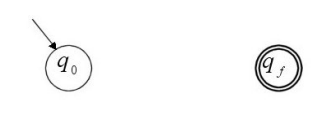
\includegraphics[scale=0.5]{imagenes/nothing}
  \end{center}
\end{figure}
\begin{figure}[H]
  \begin{center}
    \caption*{\(r=\lambda\)}
    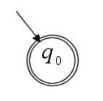
\includegraphics[scale=0.5]{imagenes/lambda}
  \end{center}
\end{figure}
\begin{figure}[H]
  \begin{center}
    \caption*{\(r=a\)}
    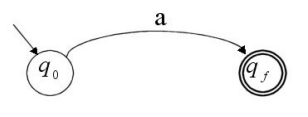
\includegraphics[scale=0.5]{imagenes/a}
  \end{center}
\end{figure}

\subsubsection{Pasos inductivos}
Sean \(r_1\) y \(r_2\) dos expresiones regulares. Supongamos que existen AFND-\(\lambda\) \\ \(M_1=\langle Q_1, \Sigma_1, \delta_1, q_1, \{f_1\}\rangle\) y \(M_2 =\langle Q_2, \Sigma_2, \delta_2, q_2, \{f_\}\rangle\) tal que \(\mathcal{L}(M_1) = \mathcal{L}(r_1)\) y \(\mathcal{L}(M_2) = \mathcal{L}(r_2)\). Vamos a armar a partir de estos autómata uno nuevo que acepte los lenguajes generados por las expresiones \(r_1|r_2\), \(r_1r_2\), \(r_1^*\) y \(r^+\).

\paragraph{\(\bm{r_1|r_2}\):} Podemos construir un automata \(M_0=\langle Q_0, \Sigma_0, \delta_0, q_0, \{f_0\}\rangle\) tal que \(\mathcal{L}(M_0) = \mathcal{L}(r_1|r_2)\) de la siguiente forma:
\begin{itemize}
  \item \(Q_0 = Q_1 \cup Q_2 \cup \{q_0, f_0\}\)
  \item \(\Sigma_0 = \Sigma_1 \cup \Sigma_2\)
  \item \(\delta_0: Q_0 \times \Sigma_0 \rightarrow \mathcal{P}(Q_0)\)
        \begin{itemize}
          \item[] \(\delta(q_0, \lambda) = \{q_1, q_2\}\)
          \item[] \(\delta(q, a) = \delta_1(q, a)\) para \(q\in Q_1-\{f_1\}\) y \(a\in \Sigma_1\cup\{\lambda\}\)
          \item[] \(\delta(q, a) = \delta_2(q, a)\) para \(q\in Q_2-\{f_2\}\) y \(a\in \Sigma_2\cup\{\lambda\}\)
          \item[] \(d(f_1,\lambda) = d(f_2,\lambda) = \{f_0\}\)
        \end{itemize}
\end{itemize}
\begin{figure}[H]
  \begin{center}
    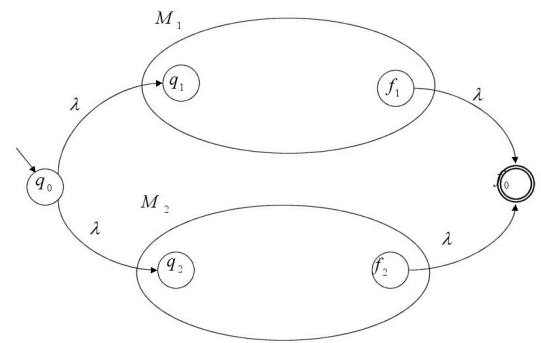
\includegraphics[scale=0.5]{imagenes/union}
  \end{center}
\end{figure}

\paragraph{\(\bm{r_1r_2}\):} \(M_0=\langle Q_0, \Sigma_0, \delta_0, q_1, \{f_2\}\rangle\):
\begin{itemize}
  \item \(Q_0 = Q_1 \cup Q_2\)
  \item \(\Sigma_0 = \Sigma_1 \cup \Sigma_2\)
  \item \(\delta_0: Q_0 \times \Sigma_0 \rightarrow \mathcal{P}(Q_0)\)
        \begin{itemize}
          \item[] \(\delta(q, a) = \delta_1(q, a)\) para \(q\in Q_1-\{f_1\}\) y \(a\in \Sigma_1\cup\{\lambda\}\)
          \item[] \(\delta(q, a) = \delta_2(q, a)\) para \(q\in Q_2-\{f_2\}\) y \(a\in \Sigma_2\cup\{\lambda\}\)
          \item[] \(d(f_1,\lambda) = \{q_2\}\)
        \end{itemize}
\end{itemize}
\begin{figure}[H]
  \begin{center}
    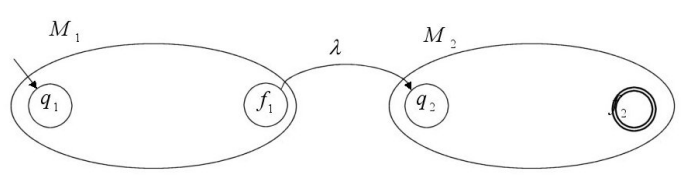
\includegraphics[scale=0.5]{imagenes/concat}
  \end{center}
\end{figure}

\paragraph{\(\bm{r_1^*}\):} \(M_0=\langle Q_0, \Sigma_1, \delta_0, q_0, \{f_0\}\rangle\):

\begin{itemize}
  \item \(Q_0 = Q_1 \cup \{f_0, q_0\}\)\
  \item \(\delta_1: Q_0 \times \Sigma_1 \rightarrow \mathcal{P}(Q_0)\)
        \begin{itemize}
          \item[] \(\delta(q_0, \lambda) = \delta(f_1,\lambda) = \{q_1, f_0\}\)
          \item[] \(\delta(q, a) = \delta_1(q, a)\) para \(q\in Q_1-\{f_1\}\) y \(a\in \Sigma_1\cup\{\lambda\}\)
        \end{itemize}
\end{itemize}
\begin{figure}[H]
  \begin{center}
    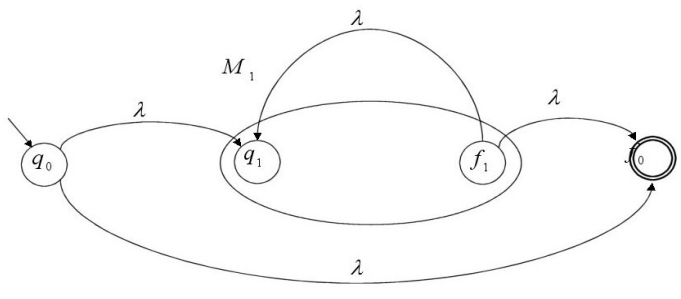
\includegraphics[scale=0.5]{imagenes/estrella}
  \end{center}
\end{figure}

Para el caso \(r_1^+\) es el mismo autómata que para este caso sin la transición \(q_0\overset{\lambda}{\rightarrow}f_0\).

\subsection{AFD a expresión regular}
\label{subsec:afd-er}
Dado un AFD \(M=\langle\{q_1, \dots, q_n\}, \Sigma, \delta, q_1, F\rangle\), que acepta el lenguaje \(\mathcal{L}\), existe una expresión regular que denota el mismo lenguaje.

\subsubsection{Demostración}
Nombremos \(R^k_{i,j}\) a la expresión regular cuyo lenguaje \(\omega \subseteq\Sigma^*\) son las cadenas que llevan al autómata \(M\) desde el estado \(q_i\) al estado \(q_j\) pasando solo por estados \(q_l\) con \(l\leq k\). En particular \(R^n_{i,j}\) es la expresión regular que representa todas las cadenas que permiten ir del estado \(i\) al estado \(j\).

Vamos a buscar como construir \(R^k_{i,j}\) para cada \(k\in\{0, \dots, n\}\) de manera inductiva. Suponiendo que demostramos la existencia de esta expresión regular, podemos concluir que la unión \(R^n_{1,f_1}|R^n_{1,f_2}|...|R^n_{1,f_m}\) (con \(f_1\dots f_m\in F\)) es la expresión regular que representa el lenguaje \(\mathcal{L}\):

\paragraph*{Caso base (\(k=0\)):} Como todos los estados están enumerados del 1 para arriba, \(k=0\) significa que no debe haber estados intermedios en el camino entre \(q_i\) y \(q_j\), por lo que pueden ser de dos formas:
\begin{itemize}
  \item Una arco del estado \(i\) al estado \(j\).
  \item Un camino de longitud cero que solo contiene el estado \(i\).
\end{itemize}

Si \(i\neq j\), entonces solo es posible la primera opción. Debemos examinar el AFD y encontrar aquellos simbolos que nos permitan ir del estado \(i\) al estado \(j\).

\begin{enumerate}
  \item Si no existe tal símbolo, entonces \(R^0_{i,j} = \varnothing\).
  \item Si existe exactamente un símbolo \(a\), entonces \(R^0_{i,j} = a\).
  \item Si existen más de un símbolo, entonces \(R^0_{i,j} = a_1|a_2|...|a_n\).
\end{enumerate}

Ahora, si \(i = j\) entonces los caminos de longitud cero también son posibles, por lo que habría que agregar a cada una de las expresiones recién mencionadas el simbolo \(\lambda\):
\begin{enumerate}
  \item \(R^0_{i,j} = \lambda\).
  \item \(R^0_{i,j} = a|\lambda\).
  \item \(R^0_{i,j} = a_1|a_2|...|a_n|\lambda\).
\end{enumerate}

\paragraph{Paso inductivo:} Supongamos que hay un camino desde el estado \(i\) al estado \(j\) que no pasa por estados mas grandes \(k\). Entonces podemos considerar las siguientes dos opciones:
\begin{enumerate}
  \item El camino no pasa por el estado \(k\), por lo que el lenguaje de \(R^{k-1}_{i,j}\) contiene a ese camino.
  \item El camino pasa por el estado \(k\) por lo menos una vez. Entonces podemos partir el camino en varias partes:
        \begin{figure}[H]
          \begin{center}
            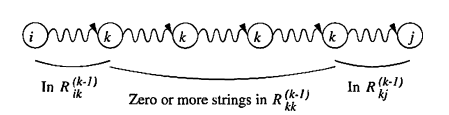
\includegraphics[scale=0.75]{imagenes/afd_regular.png}
          \end{center}
        \end{figure}
        La primer parte, va desde el estado \(i\) al estado \(k\) sin pasar por \(k\), la última parte es desde el estado \(k\) al estado \(j\) sin pasar por \(k\), y todas las partes intermedia s van desde el estado \(k\) al estado \(k\) sin pasar por \(k\). Cada una de estas partes ya tiene una expresión regular asociada: \(R^{k-1}_{i,k}\), \(R^{k-1}_{k,k}\), \(R^{k-1}_{k,j}\), por lo que podemos unirlas para obtener la expresión regular que representa el camino completo de la siguiente forma:
        \[
          R^{k-1}_{i,k}\left(R^{k-1}_{k,k}\right)^*R^{k-1}_{k,j}
        \]
\end{enumerate}

Entonces \(R^k_{i,j}\) es la unión de las expresiones de los dos tipos de caminos que acabamos de describir:
\[
  R^k_{i,j} = R^{k-1}_{i,j} \cup R^{k-1}_{i,k}\left(R^{k-1}_{k,k}\right)^*R^{k-1}_{k,j}
\]

Finalmente, si construimos en orden todas estas expresiones regulares desde \(R^0_{i,j}\), eventualmente llegaremos hasta \(R^n_{i,j}\).

Y como dijimos, más arriba si calculamos \(R^0_{1,j}\) para cada \(q_j\in F\) y unimos todas las expresiones, obtendremos la expresión regular que representa el lenguaje \(\mathcal{L}\).

\newpage
\subsection{Gramática regular a AFND}
Dada una grámatica regular \(G = \langle V_N, V_T, P, S\rangle\), podemos construir un AFND \\ \(M=\langle Q,\Sigma, \delta, q_0, F\rangle\) que reconozca el lenguaje generado por \(G\)

\subsubsection{Demostración}
Vamos a constuir el autómata finito no determinista \(M\) y demostrar que reconoce el lenguaje generado por \(G\).
\paragraph{Construcción de \(M\):} Construyamos \(M\) de la siguiente manera:
\begin{itemize}
  \item \(Q = V_N\cup\{q_f\}\). Denotarmeos \(q_A\) al estado que representa al no símbolo no terminar \(A\).
  \item \(\Sigma = V_T\)
  \item \(q_0 = q_S\)
  \item Si \(A, B \in V_N\) y \(a\in\Sigma\), entonces:
        \begin{itemize}
          \item \(q_B\in\delta(q_A, a) \iff A \rightarrow aB \in P\)
          \item \(q_f \in \delta(q_A, a) \iff A \rightarrow a \in P\)
          \item \(q_A\in F \iff A \rightarrow \lambda \in P\)
          \item \(q_f\in F\)
        \end{itemize}
\end{itemize}

\paragraph{Equivalencia clausura transitiva de producciones y \(\delta\): } Vamos a probar por inducción que
\[A   \overset{*}{\Rightarrow} \alpha B \iff q_B\in\hat\delta(q_A, \alpha)\]

\begin{itemize}
  \item \textbf{Caso base \(\alpha = \lambda\):}
        \begin{itemize}
          \item \(A\overset{*}{\Rightarrow} \alpha B\), pero las gramáticas regulares no acentan producciones que vayan de un no terminal a otro sin pasar por un terminal, por lo que \(B = A\). Osea \(A\overset{*}{\Rightarrow} \alpha A\).
          \item Además, como es un AFND, no tiene transiciones lambda, osea que \(\delta(q_A, \lambda) = \{q_A\}\), por lo que \(q_A\in\hat\delta(q_A, \alpha)\).
        \end{itemize}
  \item \textbf{Caso inductivo \(\alpha = \beta a\):}
        \begin{align*}
          A\overset{*}{\Rightarrow} \alpha B   \iff & A\overset{*}{\Rightarrow} \beta aB \iffa{def.} \red{\exists C\in V_N: A \overset{*}{\Rightarrow} \beta C} \wedge \blue{C\rightarrow aB} \\
          \iffab{\red{H.I}}{\blue{constr. M}}       & \blue{\exists q_C\in Q, q_c\in\hat\delta(q_A,\alpha)} \land \red{q_B\in\delta(q_C,a)}                                                   \\
          \iff                                      & q_B\in \delta(\hat\delta(q_A,\alpha),a)                                                                                                 \\
          \iff                                      & q_B\in\hat\delta(q_A, \beta a) \iff q_B\in\hat\delta(q_A, \alpha)                                                                       \\
        \end{align*}
\end{itemize}

\paragraph{Demostración de la equivalencia:} Vamos a demostrar que el lenguaje generado por \(G\) y \(M\) son iguales, osea que \(\alpha a\in\mathcal{L}(M)\iff S\overset{*}{\Rightarrow} \alpha a\).
Como \(G\) es una grámatica regular, hay solo dos formas de llegar desde \(S\) hasta \(\alpha a\):
\begin{enumerate}
  \item \(\exists A\in V_N: S \overset{*}{\Rightarrow} \alpha A \wedge A \rightarrow a \in P\)
  \item \(\exists B\in V_N: S \overset{*}{\Rightarrow} \alpha aB \wedge B \rightarrow \lambda \in P\)
\end{enumerate}
Entonces:

\begin{align*}
  S\overset{*}{\Rightarrow} \alpha a \iffa{def. G} & (\exists A\in V_N: S \overset{*}{\Rightarrow} \alpha A \wedge A \rightarrow a \in P)\lor(\exists B\in V_N: S \overset{*}{\Rightarrow} \alpha aB \wedge B \rightarrow \lambda \in P) \\
  \iffa{Equiv. anterior}                           & (\exists q_A\in Q, q_A\in\hat\delta(q_0, \alpha) \land q_f\in\delta(q_A, a)) \lor (\exists q_B\in Q, q_B\in\hat\delta(q_0, \alpha a) \land q_B\in F)                                \\
  \iffa{def. \(\delta\)}                           & q_f\in\delta(q_S, \alpha a) \lor (\exists q_B\in Q, q_B\in\hat\delta(q_0, \alpha a) \land q_B\in F)                                                                                 \\
  \iff                                             & \alpha a \in \mathcal{L}(M)                                                                                                                                                         \\
\end{align*}

Falta ver que pasa si \(\lambda\in\mathcal{L}(G)\):

\[ \lambda\in\mathcal{L}(G) \iff S\overset{*}{\Rightarrow} \lambda \iff S\rightarrow \lambda \in P \iff q_S\in F \iff \lambda \in \mathcal{L}(M)\]
\subsection{AFD a gramática regular}
Dado un AFD \(M=\langle Q, \Sigma, \delta, q_0, F\rangle\), existe una gramática regular \(G=\langle V_N, V_T, P, S\rangle\) equivalente

\subsubsection{Demonstración}
\paragraph{Contrucción de \(G\):} Vamos a construir \(G\) de la siguiente forma:
\begin{itemize}
  \item \(V_N = Q\), para mayor claridad llamamos \(A_p\) al no terminal correspondiente al estado \(p\in Q\)
  \item \(V_T = \Sigma\)
  \item \(S = q_0\)
  \item Si \(q\in Q \land q\notin F\) entonces \(A_p \rightarrow aA_q \in P \iff \delta(p,a) = q\)
  \item Si \(q\in F\) entonces \(A_p \rightarrow a \in P \iff \delta(p,a) = q\)
  \item \(S\rightarrow \lambda \in P \iff q_0\in F\)
\end{itemize}

\paragraph{Paso intermedio:} Vamos a demostrar por inducción: \[ \hat\delta(p,\alpha) = q \iff A_p \overset{*}{\Rightarrow} \alpha A_q\]

\begin{itemize}
  \item \textbf{Caso base:} \(\alpha = \lambda\) es trivial:
        \begin{align*}
           & \hat\delta(p,\lambda) = q \iff A_p \overset{*}{\Rightarrow} A_p
        \end{align*}
  \item \textbf{Caso inductivo \(\alpha = \beta a\):} Queremos probar que \(\hat\delta(p,\alpha) = q \iff A_p \overset{*}{\Rightarrow} \alpha A_q\).

        Nuestra hipotesis inductiva: \(\hat\delta(p,\beta) = q \iff A_p \overset{*}{\Rightarrow} \beta A_q\) para todo \(|\beta| \leq n\)

        \begin{align*}
           & \hat\delta(p, \alpha) = \hat\delta(p, \beta a) = q \iffa{def.}\blue{\exists r\in Q:~\hat\delta(p,\beta) = r} \land \red{\delta(r, a) = q}                                            \\
           & \iffab{\blue{H.I}}{\red{constr. G}} \blue{\exists A_r, A_p \overset{*}{\Rightarrow} \beta A_r} \land \red{A_r \rightarrow a A_q \in P} \iff A_p \overset{*}{\Rightarrow} \beta a A_q \\
        \end{align*}
\end{itemize}

\paragraph{Demostración de equivalencia de lenguajes:}
\begin{align*}
   & \alpha a\in\mathcal{L}(M) \iffa{def.} \hat\delta(q_0, \alpha a) \in F \iffa{def.} \exists q\in Q:~\hat\delta(q_0, \alpha) = q \land \delta(q,a)\in F                        \\
   & \underset{\text{paso intermedio}}{\iff} \exists A_p, A_{q0} \overset{*}{\Rightarrow} \alpha A_p \land A_p \rightarrow a \in P \iff A_{q0} \overset{*}{\Rightarrow} \alpha a \\
   & \underset{\text{def.}}{\iff} \alpha a \in\mathcal{L}(G)
\end{align*}


\newpage
\section{Minimización de AFD}
\subsection{Indistinguibilidad}
Sea \(M=\langle Q, \Sigma, \delta, q_0, F\rangle\) un AFD, decimos que \(p,q\in Q\),  son indistinguibles \((p\equiv q)\) si para toda cadena \(\alpha\in\Sigma^*\) tal que \(\hat\delta(p,\alpha) \in F\) entonces pasa que \(\hat\delta(q,\alpha) \in F\) y viceversa. Si \(p, q\in Q\) son indistinguibles, entonces decimos que \(p\) y \(q\) son equivalentes.

\[ p \equiv q \iff \forall \alpha \in \Sigma^*:~(\hat\delta(p,\alpha) \in F \iff \hat\delta(q,\alpha) \in F)\]

\paragraph{Teorema:} Si \(p\) y \(q\) son indistinguibles, sea \(\alpha\in\Sigma^*\) entonces \(\hat\delta(p,\alpha) \equiv \hat\delta(q,\alpha)\)

\[ p \equiv q \implies \forall \alpha \in \Sigma^*:~\hat\delta(p,\alpha) \equiv \hat\delta(q,\alpha)\]
\begin{demo}[0.8\textwidth]
  Sean \(p,q\in Q\), \(p\equiv q\).

  Supogamos que existe \(\alpha\in\Sigma^*\) tal que \(\hat\delta(p, \alpha) \not\equiv \hat\delta(q,\alpha)\) entonces existe una cadena \(\gamma\in\Sigma^*\) que distingue a \(\hat\delta(p,\alpha)\) de \(\hat\delta(q,\alpha)\). Osea que \(\hat\delta(\hat\delta(p,\alpha), \gamma) \in F\) y \(\hat\delta(\hat\delta(q,\alpha), \gamma) \not\in F\) (o viceversa).

  Por def: \(\hat\delta(\hat\delta(p,\alpha),\gamma) = \hat\delta(p,\alpha\gamma)\) y \(\hat\delta(\hat\delta(q,\alpha), \gamma) = \hat\delta(p,\alpha\gamma)\). Entonces, como \(\alpha\gamma\) es una cadena que nos permite distinguir \(p\) de \(q\), es decir \(p \not\equiv q\). Absurdo.
\end{demo}

\paragraph{Teorema:} \(\equiv\) es una relación de equivalencia.

\begin{demo}[0.8\textwidth]
  \begin{itemize}
    \item \textbf{Reflexividad:} \(p\equiv p\):
          \[ \forall \alpha \in \Sigma^*:~(\hat\delta(p,\alpha) \in F \iff \hat\delta(p,\alpha) \in F) \iff p \equiv p \]
    \item \textbf{Simetría:} \(p\equiv q \implies q\equiv p\):
          \begin{align*}
             & p \equiv q \implies \forall \alpha \in \Sigma^*:~(\hat\delta(p,\alpha) \in F \iff \hat\delta(q,\alpha) \in F)  \\
             & \iff \forall \alpha \in \Sigma^*:~(\hat\delta(q,\alpha) \in F \iff \hat\delta(p,\alpha) \in F) \iff q \equiv p
          \end{align*}
    \item \textbf{Transitividad:} \(p\equiv q \land q\equiv r \implies p\equiv r\):
          \begin{itemize}
            \item[] \(p \equiv q \implies \forall \alpha \in \Sigma^*:~(\hat\delta(p,\alpha) \in F \iff \hat\delta(q,\alpha) \in F)\)
            \item[] \(q \equiv r \implies \forall \alpha \in \Sigma^*:~(\hat\delta(q,\alpha) \in F \iff \hat\delta(r,\alpha) \in F)\)
          \end{itemize}
          Entonces
          \begin{align*}
             & \forall \alpha \in \Sigma^*:~(\hat\delta(p,\alpha) \in F \iff \hat\delta(r,\alpha) \in F) \iff p \equiv r
          \end{align*}
  \end{itemize}
\end{demo}

\subsubsection{Indestinguibilidad de orden k}
\[ p \overset{k}{\equiv} q \iff \forall \alpha\in\Sigma^*, (|\alpha|\leq k) \implies (\hat\delta(p,\alpha) \in F \iff \hat\delta(q,\alpha) \in F)\]

\paragraph{Propiedades:}
\begin{enumerate}
  \item \(\overset{k}{\equiv}\) es un relación de equivalencia.
        \begin{demo}[0.8\textwidth]
          Es exactamente igual a la demostración \(\equiv\) es transitiva.
        \end{demo}
  \item \(\overset{k+1}{\equiv}\subseteq\overset{k}{\equiv}\)
        \begin{demo}[0.8\textwidth]
          \[ p \overset{k+1}{\equiv} q \implies \forall \alpha\in\Sigma^*, (|\alpha|\leq k+1) \implies (\hat\delta(p,\alpha) \in F \iff \hat\delta(q,\alpha) \in F)\]

          Ahora como esto vale \(\forall \alpha\in\Sigma^*, (|\alpha|\leq k+1)\), necesarimente vale \(\forall \alpha\in\Sigma^*, (|\alpha|\leq k)\). Entonces
          \[ \forall \alpha\in\Sigma^*, (|\alpha|\leq k+1) \implies (\hat\delta(p,\alpha) \in F \iff \hat\delta(q,\alpha) \in F) \implies p \overset{k}{\equiv} q\]
        \end{demo}
  \item \(\left(Q / \overset{0}{\equiv}\right) = \{Q-F, F\}\) si \(Q - F \neq \emptyset\) y \(F \neq\emptyset\). En castellano, \(\overset{0}{\equiv}\) divide al conjunto de estados en estados finales y no finales.
  \item \(
        p\overset{k+1}{\equiv} q \iff \left(p \overset{0}{\equiv} q
        \right) \land \left(
        \forall a\in\Sigma, \delta(p,a) \overset{k}{\equiv} \delta(q,a)
        \right)
        \)
        \begin{demo}[0.8\textwidth]
          \begin{itemize}
            \item[\(\Rightarrow)\)] Como \(\overset{k+1}{\equiv} \subseteq \overset{k}{\equiv}\) entonces \( p\overset{k+1}{\equiv} q \implies p \overset{0}{\equiv} q\).

              Por otro lado, supongamos que no vale \(\left(
              \forall a\in\Sigma, \delta(p,a) \overset{k}{\equiv} \delta(q,a)
              \right)\) entonces
              \[
                \exists a\in\Sigma,~\exists\alpha\in\Sigma^*, (|\alpha|\leq k) \land \hat\delta(\delta(p,a), \alpha) \in F \land \hat\delta(\delta(q,a),\alpha) \notin F
              \]

              o viceversa. Pero entonces \( p \overset{k+1}{\not\equiv} q\) ya que \(a\alpha\leq k + 1 \) y \(a\alpha\) distinque a \(p\) y a \(q\).
          \end{itemize}
        \end{demo}
        \begin{demoPart}[0.8\textwidth]
          \begin{itemize}
            \item[\(\Leftarrow )\)] Supogamos que \(p \overset{k}{\equiv} q\). Entonces ó \(p \overset{0}{\equiv} q\) ó \(\exists a\alpha,~|a\alpha| \leq k + 1\) que distingue \(p\) de \(q\), o sea que:
              \[
                \hat\delta(\delta(p,a),\alpha)\in F \land \hat\delta(\delta(q,a),\alpha)\notin F
              \]

              o viceversa. Pero entonce \(\delta(p,a) \overset{k+1}{\not\equiv} \delta(q,a)\).
          \end{itemize}
        \end{demoPart}
  \item \(\left(\overset{k+1}{\equiv} = \overset{k}{\equiv}\right) \implies \forall n\geq 0, \left(
        \overset{k+n}{\equiv} = \overset{k}{\equiv}
        \right)
        \)
        \begin{demo}[0.8\textwidth]
          Lo vamos a demostrar por inducción:
          \begin{itemize}
            \item[] \textbf{Caso base:}\(n=0\). Entonces \(k \overset{k}{\equiv}=\overset{k}{\equiv}\).
            \item[] \textbf{Paso inductivo:} Suponemos que es cierto para \(n\), osea que vale \(\overset{k+1}{\equiv} =\overset{k}{\equiv} \implies \overset{k+n}{\equiv} = \overset{k}{\equiv}\)

              Queremos probar \(\overset{k+1}{\equiv} =\overset{k}{\equiv} \implies \overset{k+n+1}{\equiv} = \overset{k}{\equiv}\):

              Sabemos que \(\overset{k+n+1}{\equiv} = \overset{k}{\equiv}\) si y solo si \(\forall p,q\in Q, \left(
              p\overset{k}{\equiv} q \iff p\overset{k+n+1}{\equiv} q
              \right)\)

              Por la propiedad (4), tenemos:
              \begin{align*}
                p\overset{k+n+1}{\equiv} \iff       & \left(p \overset{0}{\equiv}q\right)\land\left(
                \forall a\in\Sigma, \delta(p,a) \overset{k+n}{\equiv} \delta(q,a)
                \right)   \left(p \overset{0}{\equiv}q\right)                                                                                                           \\ &\land\left(
                \forall a\in\Sigma, \delta(p,a) \overset{k+n}{\equiv} \delta(q,a)
                \right)                                                                                                                                                 \\
                \underset{\text{prop. 2}}{\implies} & \left(p \overset{0}{\equiv}q\right)\land\left(
                \forall a\in\Sigma, \delta(p,a) \overset{k}{\equiv} \delta(q,a) \right)                                                                                 \\
                                                    & \underset{\text{prop. 4}}{\implies} p \overset{k+1}{\equiv}q \underset{\text{prop. 2}}{\implies} q \overset{k}{p}
              \end{align*}
          \end{itemize}
        \end{demo}
\end{enumerate}
\subsection{Autómatas finito determinístico mínimo}
Sea \(M=\langle Q, \Sigma, \delta, q_0, F\rangle\) un AFD sin estados inaccesibles, el AFD mínimo equivalente \(M'= \langle Q', \Sigma, \delta', q_0, F'\rangle\) se define de la siguiente manera:
\begin{itemize}
  \item \(Q' = Q / \equiv\). Vamos a notar \([q]\) al estado que representa a la clase de equivalencia que contiene a \(q\).
  \item \(\delta'([q], a) = [\delta(q,a)]\)
  \item \(q_0' = [q_0]\)
  \item \(F' = \{[q]\in Q'~:~ q \in F\}\)
\end{itemize}

\paragraph{Teorema:}
\[\forall \alpha\in\Sigma^*, \hat\delta(q, \alpha) = r \implies \hat\delta'(q_0', \alpha) = \hat\delta'([q], \alpha) = [r]\]

\begin{demo}[0.8\textwidth]
  Va a ser por inducción en la longitud de \(\alpha\):
  \begin{itemize}
    \item \(\alpha = \lambda\): \(\hat\delta(q, \epsilon) = q\), por def. de \(\hat\delta\)

          \(\hat\delta'(q_0', \epsilon) = \hat\delta'([q], \epsilon) = [q]\) por def. de \(\hat\delta'\)

          Entonces \(\hat\delta(q, \lambda) = q \implies \hat\delta'([q], \lambda) = [q]\)
    \item Paso inductivo: Sea \(\alpha = \beta a\), queremos probar que \(\hat\delta(q,\alpha) = r \implies \hat\delta'([q], \alpha) = [r]\).

          Nuestra hipotesis inductiva es \(\forall \beta\in\Sigma^*,~|\beta|\leq n,~\hat\delta(q, \beta) = p \implies \hat\delta'([q], \beta) = [p]\)

          Entonces:

          \[ \hat\delta(q, \alpha) = \hat\delta(q, \beta a) = \delta(\hat\delta(q, \beta), a) = \hat\delta(p, a) = r \underbrace{\implies}_{\text{constr. }\delta'} \delta'([p], a) = [r] ~(1)\]

          Además, por hipotesis inductiva sabemos que \(\hat\delta'([q], \beta) = [p]\), entonces remplazando en el último término de la ecuación (1) obtenemos:

          \[ \delta'([p], \alpha) = \delta'(\hat\delta'([q], \beta), a) = \hat\delta(q,\beta a) = \hat\delta(q,\alpha) = [r] \]
  \end{itemize}

\end{demo}
\subsection{Algoritmo de minimización de un AFD}
\begin{algorithmic}
  \Require \(M = \langle Q, \Sigma, \delta, q_0, F\rangle\)
  \State \(P\leftarrow\{Q-F, F\}\) \Comment{\(P = \overset{0}{\equiv}\), separamos los estados finales de los no finales}
  \State \(stop\leftarrow false\)
  \While{\(stop = false\)}
  \State\(P'\leftarrow\emptyset\)
  \For{\(X\in P\)} \Comment{Separamos cada clase de equivalencia en las subclases de \(\overset{n+1}{\equiv}\)}
  \While{\(\exists e\in X : \lnot\texttt{marked}(e, X)\)} \Comment{Elegimos un nuevo representante para cada clase}
  \State\(X_1\leftarrow\{e\}\)
  \State\(\texttt{marked}(e,X)\)
  \For{\(e'\in X: e\neq e'\)} \Comment{Conseguimos los elementos de esa clase}
  \If{\(\lnot\texttt{marked}(e', X)\land(\forall a\in\Sigma,~[\delta(e,a)] = [\delta(e',a)])\)}
  \State\(X_1\leftarrow X_1\cup\{e'\}\)
  \State\(\texttt{mark}(e',X)\)
  \EndIf
  \EndFor
  \State \(P'\leftarrow P'\cup \{X_1\}\)
  \EndWhile
  \EndFor
  \If{\(P \neq P'\)}
  \State \(P\leftarrow P'\)
  \Else
  \State \(stop\leftarrow true\)
  \EndIf
  \EndWhile
\end{algorithmic}

\paragraph{Lema:} Sean \(M=\langle Q, \Sigma, \delta, q_0, F\rangle\) y \(M'=\langle Q', \Sigma, \delta', q'_0, F'\rangle\) dos AFDs. Si \(M\) no poseee estados inaccesibles y todo par de cadenas que conducen a estados diferentes de \(M\) conducen a estados diferentes de \(M'\), entonces la cantidad de estados de \(M'\) es mayor o igual a la cantidad de estados de \(M\). Es decir:

\[
  \left(
  \forall\alpha,\beta\in\Sigma^*,~\hat\delta(q, \alpha) \neq \hat\delta(q, \beta) \implies \hat\delta'(q_0', \alpha) \neq \hat\delta'(q_0', \beta)
  \right) \implies |Q|\leq |Q'|
\]

\begin{demo}[0.8\textwidth]
  Sea \(g:Q\to\Sigma^*\) definida por \(g(q) = \min\left\{\alpha\in\Sigma^*:~\hat\delta(q_0,\alpha) = q\right\}\) donde suponemos una relación de orden en \(\Sigma^*\) dada por la longitud para cadenas de distinta longitud, y por el lexicográfico para las cadenas de igual longitud. Definamos \(f: Q\to Q'\) con \(f(q)=\hat\delta'(q_0', g(q))\).

  Como para cualquier par de estados diferentes \(p,q\in Q\) es cierto que \(\hat\delta(q_0, g(p))\neq\hat\delta(q_0, g(q))\), entonces \(\hat\delta'(q_0', g(p))\neq\hat\delta'(q_0', g(q))\). Lo que equivale a decir que \(f(p)\neq f(q)\). Por lo tanto, \(f\) es una función inyectiva, es decir que \(|Q|\leq |Q'|\).
\end{demo}

\paragraph{Lema:} Sea \(M_R = \langle Q_R, \Sigma, \delta_R, q_{R0}, F_R\rangle\) el autómata reducido correspondiente a \\ \(M = \langle Q, \Sigma, \delta, q_0, F\rangle\). Entonces, cualquier autómata \(M' = \langle Q', \Sigma, \delta', q_{0'}, F'\rangle\) que reconozca el mismo lenguaje que \(M\) no poseerá menos estados que \(M_R\). Osea:
\[
  \forall M',~\mathcal{L} (M') = \mathcal{L} (M) \implies |Q'| \geq |Q_R|
\]

\begin{demo}[0.8\textwidth]
  Supongamos que \(\exists M'\) tal que \( |Q'| < |Q_R|\), entonces según el lema anterior deben existir dos cadenas \(\alpha,\beta\in\Sigma^*\) tales que
  \[
    \hat{\delta_R}(q_0,\alpha) \neq \hat{\delta_R}(q_0,\beta) \land \hat{\delta'}(q_0',\alpha) = \hat{\delta'}(q_0',\beta)
  \]
  Pero entonces, como \(\hat{\delta_R}(q_0,\alpha)\) y \(\hat{\delta_R}(q_0,\beta)\) son estados diferentes, entonces \(\hat{\delta}(q_0,\alpha)\) y \(\hat{\delta}(q_0,\beta)\) son estados distinguibles por pertenecer al autómata reducido \(M_R\) entonces \(\exists\gamma\in\Sigma^*\) tal que:
  \[
    \hat{\delta}(q_0,\alpha\gamma)\in F \land \hat{\delta}(q_0,\beta\gamma)\notin F
  \]
  o viceversa. Entonces \(\alpha\gamma\in\mathcal{L}(M_R) \iff \beta\gamma\notin\mathcal{L}(M_R)\).

  Por otro lado, como \(\hat\delta'(q_0',\alpha) = \hat\delta'(q_0',\beta)\), es obvio que \[
    \hat\delta'(q_0',\alpha\gamma)\in F\land \hat\delta'(q_0',\beta\gamma)\in F
  \] o ninguno de los dos perteneces a \(F\). De esto se inifiere que \(\alpha\gamma\in\mathcal{L}(M') \iff \beta\gamma\in\mathcal{L}(M')\).

  Pero entonces, \(\mathcal{L}(M') \neq \mathcal{L}(M)\), se contradice nuestra hipotesis inicial.
\end{demo}

\newpage
\section{Lenguajes regulares y lema de pumping}
\label{sec:pumping}
\subsection{Lema de pumping}
\label{subsec:pumping}
\paragraph{Propiedad:} Sea \(\mathcal{L}\) un lenguaje regular, si las longitudes de las cadenas de un lenguaje \(\mathcal{L}\) están acotadas superiormente, entonces \(\mathcal{L}\) tiene que ser finito.

\paragraph{Propiedad:} Si \(\mathcal{L}\) es un luenguaje regular infinito, entonces el grafo de un autómata fínito que acepte \(\mathcal{L}\) tiene que tener un camino desde el estado inicial hasta algún estado final que paso por algún ciclo.

\paragraph{Lema de pumping:} Sea \(\mathcal{L}\) un lenguaje regular, si \(\mathcal{L}\) es infinito, entonces todas las cadenas \(\omega\) de longitud mayor o igual a \(n\) (para algún \(n > 1\)) van a ser de la forma \(\omega=xy^iz\), estext decir hay una parte de \(\omega\) que se repite \(i\) cantidad de veces:

\begin{align*}
   & \mathcal{L} \text{ es regular e infinito}\implies \exists n\in\mathbb{N}\text{ tal que } \\ &\forall\omega\in\mathcal{L},~|\omega|\geq n:\left( \exists x,y,z\in\Sigma^*: \omega=xyz\land|xy|\leq n\land|z|\geq 1 \land (\forall i\geq  0 :~ xy^iz\in\mathcal{L}\right) \\
\end{align*}
\begin{demo}[0.8\textwidth]  Supongamos que \(\mathcal{L}\) es un lenguaje regular. Entonces existe una AFD \(A =\langle Q, \Sigma, \delta, q_0, F\rangle\) que acepta \(\mathcal{L}\).

  Sea \(n = |Q|\) la cantidad de estados de \(A\) y \(\omega=a_1a_2\dots a_m\in\Sigma^*\) de longitud \(m > n\). Para cada \(i = 0,\dots, m\) definamos el estado \(p_i = \hat\delta(q_0, a_1\dots a_i)\) (el estado en el que se encuentra \(A\) después de haber consumido los primeros \(i\) símbolos de \(\omega\).

  Como el \(A\) solo tiene \(n\) estados pero hay \(m > n\) estados \(p\), poes imposible que todos los \(p\) sean distintos. Por lo tanto, existen \(0 \leq i < j \leq n\) tales que \(p_i = p_j\).

  Considerar entonces la siguiente descomposición para \(\omega = xyz\):
  \begin{itemize}
    \item[] \(x = a_1\dots a_i\)
    \item[] \(y = a_{i+1}\dots a_j\)
    \item[] \(z = a_{j+1}\dots a_m\)
  \end{itemize}
  Entonces podemos concluir que:
  \begin{itemize}
    \item[] \(\hat\delta(q_0, x) = p_j\)
    \item[] \(\hat\delta(p_i, y) = p_j\) (que como son el mismo estado implica que \(A\) tiene un ciclo)
    \item[] \(\hat\delta(p_j, z) = p_m\)
  \end{itemize}

\end{demo}
\begin{demoPart}[0.8\textwidth]

  Observar que \(x\) podría ser la cadena cuando \(i = 0\), \(z\) podría ser vacía si \(j = n = m\), pero \(y\) no puede ser vacía ya que se tomó \(i < j\).

  Vimos entonces que si \(\mathcal{L}\) es regular y \(|\omega| \geq n\) entonces podemos dividirla en cadenas \(x,y,z\) tal que \(|xy|\leq n\) y \(|z|\geq 1\). Ahora vamos a ver que si \(xyz \in \mathcal{L}\) entonces \(xy^kz \in \mathcal{L}\) para todo \(k\geq 0\).

  \begin{itemize}
    \item Si \(k = 0\) entonces \(xy^0z = xz\):
          \[\hat\delta(q_0, xz) = \hat\delta(\hat\delta(q_0, x), z) = \hat\delta(p_i, z) = \hat\delta(p_j, z) = p_m\]
          Y \(p_m\) es un estado final pues es el mismo estado al que llegamos si la entrada fuese \(xyz\in\mathcal{L}\). Entonces \(xz = xy^0z \in \mathcal{L}\).
    \item Si \(i > 0\). Entonces \(A\) consume \(x\) desde \(q_0\) y llega hasta \(p_i\). Luego \(A\) consume \(y\) desde \(p_i\) y llega hasta \(p_j\) (que son iguales) y repite este ciclo \(k\) veces hasta consumir todas las apariciones de \(y\) en la cadena. Finalmente \(A\) consume \(z\) desde \(p_j\) y llega hasta \(p_m\). Entonces \(A\) llega a un estado final y por lo tanto \(xy^kz \in \mathcal{L}\).
  \end{itemize}
\end{demoPart}
\paragraph{Contrarecíproco:}
\begin{align*}
   & \forall   n\in\mathbb{N}  \exists\omega\in\mathcal{L}\text{ tal que } |\omega|\geq n \land  \forall x,y,z\in\Sigma^*: \omega\neq xyz \land|xy|\geq n\lor|z|\leq 1 \lor \exists i\geq 0,~ xy^iz\notin\mathcal{L} \\ &
  \implies \mathcal{L}\text{  no es regular}                                                                                                                                                                         \\
\end{align*}
\end{document}